%%%%%%%%%%%%%%%%%%%%%%%%%%%%%%%%%%%%%%%%%%%%%%%%%%%%%%%%%%%%%%%%%%%%%%%%%%%%%%%%%%%%%%%%%%%%%%%%%
%
% Document:     Data Management  product tree
%
%%%%%%%%%%%%%%%%%%%%%%%%%%%%%%%%%%%%%%%%%%%%%%%%%%%%%%%%%%%%%%%%%%%%%%%%%%%%%%
\documentclass{article}
\usepackage{times,layouts}
\usepackage{tikz,hyperref,amsmath}
\usetikzlibrary{positioning,arrows,shapes,decorations.shapes,shapes.arrows}
\usetikzlibrary{backgrounds,calc}
\usepackage[paperwidth=26.0cm,paperheight=145.58cm,
left=-2mm,top=3mm,bottom=0mm,right=0mm,
noheadfoot,marginparwidth=0pt,includemp=false,
textwidth=30cm,textheight=50mm]{geometry}
\newcommand\showpage{%
\setlayoutscale{0.5}\setlabelfont{\tiny}\printheadingsfalse\printparametersfalse
\currentpage\pagedesign}
\hypersetup{pdftitle={DM products }, pdfsubject={Diagram illustrating the
                products in LSST DM }, pdfauthor={Autogenerated from MD}}
\tikzstyle{tbox}=[rectangle,text centered, text width=30mm]
\tikzstyle{wbbox}=[rectangle, rounded corners=3pt, draw=black, top color=blue!50!white,
                    bottom color=white, very thick, minimum height=12mm, inner sep=2pt,
                    text centered, text width=30mm]
\tikzstyle{pbox}=[rectangle, rounded corners=3pt, draw=black, top
 color=yellow!50!white, bottom color=white, very thick,
 minimum height=35pt, inner sep=2pt, text centered, text width=35mm]
\tikzstyle{pline}=[-, thick]
\begin{document}
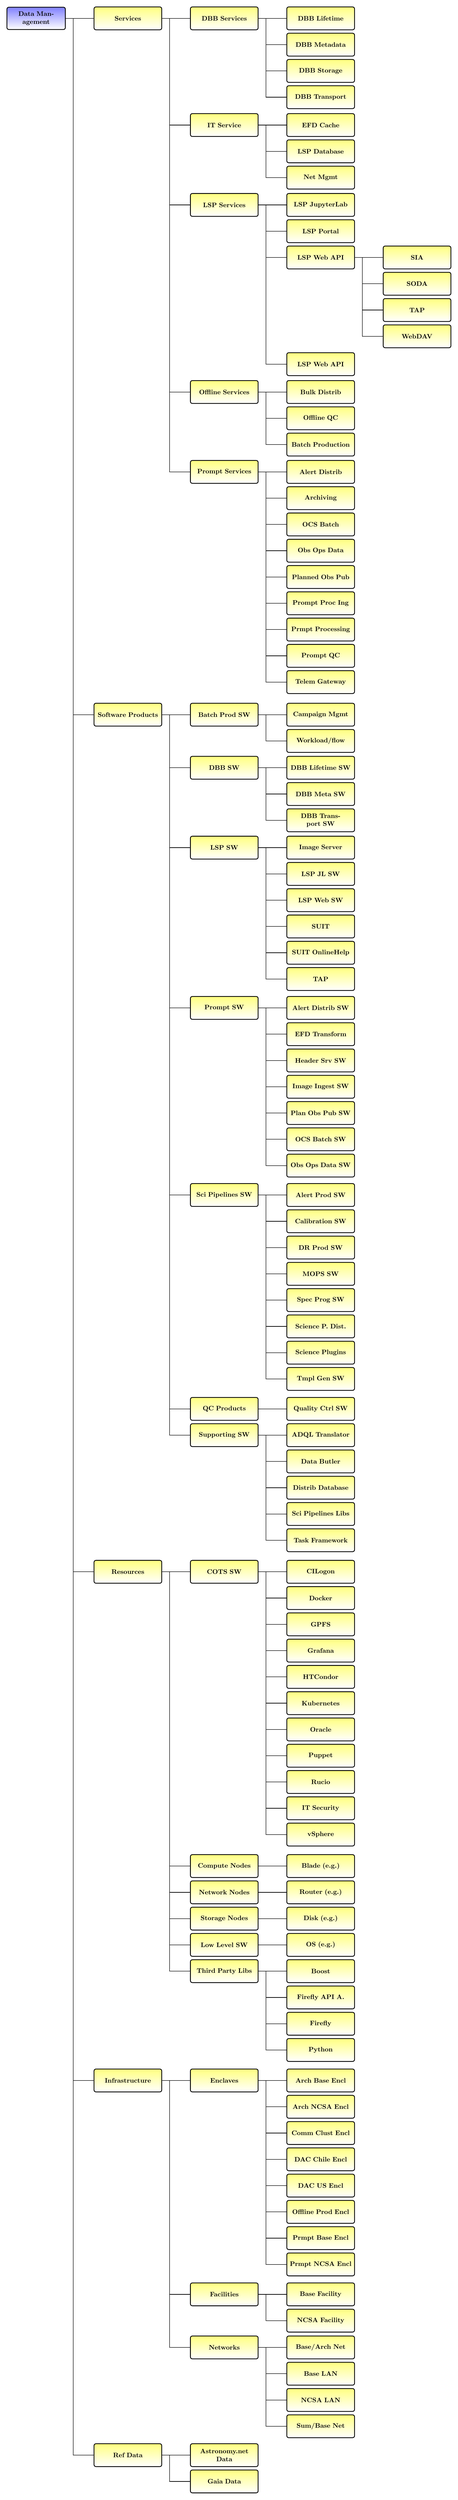
\begin{tikzpicture}[node distance=0mm]


\node (DM) [wbbox]{\textbf{Data Management}};
\node (DMSRV) [pbox,right=15mm of DM] {\textbf{Services} };
 \draw[pline] (DM.east) -| ++(0.4,0) |- (DMSRV.west); 
\node (DBBSRV) [pbox,right=15mm of DMSRV] {\textbf{DBB Services} };
 \draw[pline] (DMSRV.east) -| ++(0.4,0) |- (DBBSRV.west); 
\node (DBBLIFESRV) [pbox,right=15mm of DBBSRV] {\textbf{DBB Lifetime} };
 \draw[pline] (DBBSRV.east) -| ++(0.4,0) |- (DBBLIFESRV.west); 
\node (DBBMDSRV) [pbox,below=4pt of DBBLIFESRV] {\textbf{DBB Metadata} };
 \draw[pline] (DBBSRV.east) -| ++(0.4,0) |- (DBBMDSRV.west); 
\node (DBBSTRSRV) [pbox,below=4pt of DBBMDSRV] {\textbf{DBB Storage} };
 \draw[pline] (DBBSRV.east) -| ++(0.4,0) |- (DBBSTRSRV.west); 
\node (DBBTRSRV) [pbox,below=4pt of DBBSTRSRV] {\textbf{DBB Transport} };
 \draw[pline] (DBBSRV.east) -| ++(0.4,0) |- (DBBTRSRV.west); 
\node (ITSRV) [pbox,below=127pt of DBBSRV] {\textbf{IT Service} };
 \draw[pline] (DMSRV.east) -| ++(0.4,0) |- (ITSRV.west); 
\node (EFDB) [pbox,right=15mm of ITSRV] {\textbf{EFD Cache} };
 \draw[pline] (ITSRV.east) -| ++(0.4,0) |- (EFDB.west); 
\node (LSPDB) [pbox,below=4pt of EFDB] {\textbf{LSP Database} };
 \draw[pline] (ITSRV.east) -| ++(0.4,0) |- (LSPDB.west); 
\node (NETMGMT) [pbox,below=4pt of LSPDB] {\textbf{Net Mgmt} };
 \draw[pline] (ITSRV.east) -| ++(0.4,0) |- (NETMGMT.west); 
\node (LSPSRV) [pbox,below=86pt of ITSRV] {\textbf{LSP Services} };
 \draw[pline] (DMSRV.east) -| ++(0.4,0) |- (LSPSRV.west); 
\node (LSPJLSRV) [pbox,right=15mm of LSPSRV] {\textbf{LSP JupyterLab} };
 \draw[pline] (LSPSRV.east) -| ++(0.4,0) |- (LSPJLSRV.west); 
\node (LSPPRTLSRV) [pbox,below=4pt of LSPJLSRV] {\textbf{LSP Portal} };
 \draw[pline] (LSPSRV.east) -| ++(0.4,0) |- (LSPPRTLSRV.west); 
\node (LSPWAPI) [pbox,below=4pt of LSPPRTLSRV] {\textbf{LSP Web API} };
 \draw[pline] (LSPSRV.east) -| ++(0.4,0) |- (LSPWAPI.west); 
\node (SIASRV) [pbox,right=15mm of LSPWAPI] {\textbf{SIA} };
 \draw[pline] (LSPWAPI.east) -| ++(0.4,0) |- (SIASRV.west); 
\node (SODA) [pbox,below=4pt of SIASRV] {\textbf{SODA} };
 \draw[pline] (LSPWAPI.east) -| ++(0.4,0) |- (SODA.west); 
\node (TAPSEV) [pbox,below=4pt of SODA] {\textbf{TAP} };
 \draw[pline] (LSPWAPI.east) -| ++(0.4,0) |- (TAPSEV.west); 
\node (WDAV) [pbox,below=4pt of TAPSEV] {\textbf{WebDAV} };
 \draw[pline] (LSPWAPI.east) -| ++(0.4,0) |- (WDAV.west); 
\node (LSPWEBSRV) [pbox,below=127pt of LSPWAPI] {\textbf{LSP Web API} };
 \draw[pline] (LSPSRV.east) -| ++(0.4,0) |- (LSPWEBSRV.west); 
\node (OFFLSRV) [pbox,below=250pt of LSPSRV] {\textbf{Offline Services} };
 \draw[pline] (DMSRV.east) -| ++(0.4,0) |- (OFFLSRV.west); 
\node (BULKDSRV) [pbox,right=15mm of OFFLSRV] {\textbf{Bulk Distrib} };
 \draw[pline] (OFFLSRV.east) -| ++(0.4,0) |- (BULKDSRV.west); 
\node (OFFLQCSRV) [pbox,below=4pt of BULKDSRV] {\textbf{Offline QC} };
 \draw[pline] (OFFLSRV.east) -| ++(0.4,0) |- (OFFLQCSRV.west); 
\node (PRODSRV) [pbox,below=4pt of OFFLQCSRV] {\textbf{Batch Production} };
 \draw[pline] (OFFLSRV.east) -| ++(0.4,0) |- (PRODSRV.west); 
\node (PRSRV) [pbox,below=86pt of OFFLSRV] {\textbf{Prompt Services} };
 \draw[pline] (DMSRV.east) -| ++(0.4,0) |- (PRSRV.west); 
\node (ALRTDSTSRV) [pbox,right=15mm of PRSRV] {\textbf{Alert Distrib} };
 \draw[pline] (PRSRV.east) -| ++(0.4,0) |- (ALRTDSTSRV.west); 
\node (ARCSRV) [pbox,below=4pt of ALRTDSTSRV] {\textbf{Archiving} };
 \draw[pline] (PRSRV.east) -| ++(0.4,0) |- (ARCSRV.west); 
\node (OCSBATSRV) [pbox,below=4pt of ARCSRV] {\textbf{OCS Batch} };
 \draw[pline] (PRSRV.east) -| ++(0.4,0) |- (OCSBATSRV.west); 
\node (OODSSRV) [pbox,below=4pt of OCSBATSRV] {\textbf{Obs Ops Data} };
 \draw[pline] (PRSRV.east) -| ++(0.4,0) |- (OODSSRV.west); 
\node (POPSRV) [pbox,below=4pt of OODSSRV] {\textbf{Planned Obs Pub} };
 \draw[pline] (PRSRV.east) -| ++(0.4,0) |- (POPSRV.west); 
\node (PRPINGSRV) [pbox,below=4pt of POPSRV] {\textbf{Prompt Proc Ing} };
 \draw[pline] (PRSRV.east) -| ++(0.4,0) |- (PRPINGSRV.west); 
\node (PRPRSRV) [pbox,below=4pt of PRPINGSRV] {\textbf{Prmpt Processing} };
 \draw[pline] (PRSRV.east) -| ++(0.4,0) |- (PRPRSRV.west); 
\node (PRQCSRV) [pbox,below=4pt of PRPRSRV] {\textbf{Prompt QC} };
 \draw[pline] (PRSRV.east) -| ++(0.4,0) |- (PRQCSRV.west); 
\node (TMGSRV) [pbox,below=4pt of PRQCSRV] {\textbf{Telem Gateway} };
 \draw[pline] (PRSRV.east) -| ++(0.4,0) |- (TMGSRV.west); 
\node (DMSW) [pbox,below=1029pt of DMSRV] {\textbf{Software Products} };
 \draw[pline] (DM.east) -| ++(0.4,0) |- (DMSW.west); 
\node (BPP) [pbox,right=15mm of DMSW] {\textbf{Batch Prod SW} };
 \draw[pline] (DMSW.east) -| ++(0.4,0) |- (BPP.west); 
\node (CMPGN) [pbox,right=15mm of BPP] {\textbf{Campaign Mgmt} };
 \draw[pline] (BPP.east) -| ++(0.4,0) |- (CMPGN.west); 
\node (WLWF) [pbox,below=4pt of CMPGN] {\textbf{Workload/flow} };
 \draw[pline] (BPP.east) -| ++(0.4,0) |- (WLWF.west); 
\node (DBB) [pbox,below=45pt of BPP] {\textbf{DBB SW} };
 \draw[pline] (DMSW.east) -| ++(0.4,0) |- (DBB.west); 
\node (DBBLIFE) [pbox,right=15mm of DBB] {\textbf{DBB Lifetime SW} };
 \draw[pline] (DBB.east) -| ++(0.4,0) |- (DBBLIFE.west); 
\node (DBBMD) [pbox,below=4pt of DBBLIFE] {\textbf{DBB Meta SW} };
 \draw[pline] (DBB.east) -| ++(0.4,0) |- (DBBMD.west); 
\node (DBBTR) [pbox,below=4pt of DBBMD] {\textbf{DBB Transport SW} };
 \draw[pline] (DBB.east) -| ++(0.4,0) |- (DBBTR.west); 
\node (LSP) [pbox,below=86pt of DBB] {\textbf{LSP SW} };
 \draw[pline] (DMSW.east) -| ++(0.4,0) |- (LSP.west); 
\node (DAXIMG) [pbox,right=15mm of LSP] {\textbf{Image Server} };
 \draw[pline] (LSP.east) -| ++(0.4,0) |- (DAXIMG.west); 
\node (LSPJL) [pbox,below=4pt of DAXIMG] {\textbf{LSP JL SW} };
 \draw[pline] (LSP.east) -| ++(0.4,0) |- (LSPJL.west); 
\node (LSPWEB) [pbox,below=4pt of LSPJL] {\textbf{LSP Web SW} };
 \draw[pline] (LSP.east) -| ++(0.4,0) |- (LSPWEB.west); 
\node (SUIT) [pbox,below=4pt of LSPWEB] {\textbf{SUIT} };
 \draw[pline] (LSP.east) -| ++(0.4,0) |- (SUIT.west); 
\node (SUITOH) [pbox,below=4pt of SUIT] {\textbf{SUIT OnlineHelp} };
 \draw[pline] (LSP.east) -| ++(0.4,0) |- (SUITOH.west); 
\node (TAPSW) [pbox,below=4pt of SUITOH] {\textbf{TAP} };
 \draw[pline] (LSP.east) -| ++(0.4,0) |- (TAPSW.west); 
\node (PR) [pbox,below=209pt of LSP] {\textbf{Prompt SW} };
 \draw[pline] (DMSW.east) -| ++(0.4,0) |- (PR.west); 
\node (ALRTDSTR) [pbox,right=15mm of PR] {\textbf{Alert Distrib SW} };
 \draw[pline] (PR.east) -| ++(0.4,0) |- (ALRTDSTR.west); 
\node (EFDT) [pbox,below=4pt of ALRTDSTR] {\textbf{EFD Transform} };
 \draw[pline] (PR.east) -| ++(0.4,0) |- (EFDT.west); 
\node (HEADER) [pbox,below=4pt of EFDT] {\textbf{Header Srv SW} };
 \draw[pline] (PR.east) -| ++(0.4,0) |- (HEADER.west); 
\node (IIP) [pbox,below=4pt of HEADER] {\textbf{Image Ingest SW} };
 \draw[pline] (PR.east) -| ++(0.4,0) |- (IIP.west); 
\node (OBSPUB) [pbox,below=4pt of IIP] {\textbf{Plan Obs Pub SW} };
 \draw[pline] (PR.east) -| ++(0.4,0) |- (OBSPUB.west); 
\node (OCSBAT) [pbox,below=4pt of OBSPUB] {\textbf{OCS Batch SW} };
 \draw[pline] (PR.east) -| ++(0.4,0) |- (OCSBAT.west); 
\node (OODS) [pbox,below=4pt of OCSBAT] {\textbf{Obs Ops Data SW} };
 \draw[pline] (PR.east) -| ++(0.4,0) |- (OODS.west); 
\node (PRODN) [pbox,below=250pt of PR] {\textbf{Sci Pipelines SW} };
 \draw[pline] (DMSW.east) -| ++(0.4,0) |- (PRODN.west); 
\node (APPRMPT) [pbox,right=15mm of PRODN] {\textbf{Alert Prod SW} };
 \draw[pline] (PRODN.east) -| ++(0.4,0) |- (APPRMPT.west); 
\node (DMCAL) [pbox,below=4pt of APPRMPT] {\textbf{Calibration SW} };
 \draw[pline] (PRODN.east) -| ++(0.4,0) |- (DMCAL.west); 
\node (DRP) [pbox,below=4pt of DMCAL] {\textbf{DR Prod SW} };
 \draw[pline] (PRODN.east) -| ++(0.4,0) |- (DRP.west); 
\node (MOPS) [pbox,below=4pt of DRP] {\textbf{MOPS SW} };
 \draw[pline] (PRODN.east) -| ++(0.4,0) |- (MOPS.west); 
\node (SP) [pbox,below=4pt of MOPS] {\textbf{Spec Prog SW} };
 \draw[pline] (PRODN.east) -| ++(0.4,0) |- (SP.west); 
\node (SPDIST) [pbox,below=4pt of SP] {\textbf{Science P. Dist.} };
 \draw[pline] (PRODN.east) -| ++(0.4,0) |- (SPDIST.west); 
\node (SPLUG) [pbox,below=4pt of SPDIST] {\textbf{Science Plugins} };
 \draw[pline] (PRODN.east) -| ++(0.4,0) |- (SPLUG.west); 
\node (TMPLGEN) [pbox,below=4pt of SPLUG] {\textbf{Tmpl Gen SW} };
 \draw[pline] (PRODN.east) -| ++(0.4,0) |- (TMPLGEN.west); 
\node (QC) [pbox,below=291pt of PRODN] {\textbf{QC Products} };
 \draw[pline] (DMSW.east) -| ++(0.4,0) |- (QC.west); 
\node (QCSW) [pbox,right=15mm of QC] {\textbf{Quality Ctrl SW} };
 \draw[pline] (QC.east) -| ++(0.4,0) |- (QCSW.west); 
\node (SUPPSW) [pbox,below=4pt of QC] {\textbf{Supporting SW} };
 \draw[pline] (DMSW.east) -| ++(0.4,0) |- (SUPPSW.west); 
\node (ADQL) [pbox,right=15mm of SUPPSW] {\textbf{ADQL Translator} };
 \draw[pline] (SUPPSW.east) -| ++(0.4,0) |- (ADQL.west); 
\node (BUTLER) [pbox,below=4pt of ADQL] {\textbf{Data Butler} };
 \draw[pline] (SUPPSW.east) -| ++(0.4,0) |- (BUTLER.west); 
\node (QSERV) [pbox,below=4pt of BUTLER] {\textbf{Distrib Database} };
 \draw[pline] (SUPPSW.east) -| ++(0.4,0) |- (QSERV.west); 
\node (SCIPIPE) [pbox,below=4pt of QSERV] {\textbf{Sci Pipelines Libs} };
 \draw[pline] (SUPPSW.east) -| ++(0.4,0) |- (SCIPIPE.west); 
\node (TXF) [pbox,below=4pt of SCIPIPE] {\textbf{Task Framework} };
 \draw[pline] (SUPPSW.east) -| ++(0.4,0) |- (TXF.west); 
\node (HWCOTS) [pbox,below=1275pt of DMSW] {\textbf{Resources} };
 \draw[pline] (DM.east) -| ++(0.4,0) |- (HWCOTS.west); 
\node (COTS) [pbox,right=15mm of HWCOTS] {\textbf{COTS SW} };
 \draw[pline] (HWCOTS.east) -| ++(0.4,0) |- (COTS.west); 
\node (CILOGON) [pbox,right=15mm of COTS] {\textbf{CILogon} };
 \draw[pline] (COTS.east) -| ++(0.4,0) |- (CILOGON.west); 
\node (DOCKER) [pbox,below=4pt of CILOGON] {\textbf{Docker} };
 \draw[pline] (COTS.east) -| ++(0.4,0) |- (DOCKER.west); 
\node (GPFS) [pbox,below=4pt of DOCKER] {\textbf{GPFS} };
 \draw[pline] (COTS.east) -| ++(0.4,0) |- (GPFS.west); 
\node (GRAFANA) [pbox,below=4pt of GPFS] {\textbf{Grafana} };
 \draw[pline] (COTS.east) -| ++(0.4,0) |- (GRAFANA.west); 
\node (HTCONDOR) [pbox,below=4pt of GRAFANA] {\textbf{HTCondor} };
 \draw[pline] (COTS.east) -| ++(0.4,0) |- (HTCONDOR.west); 
\node (K8S) [pbox,below=4pt of HTCONDOR] {\textbf{Kubernetes} };
 \draw[pline] (COTS.east) -| ++(0.4,0) |- (K8S.west); 
\node (ORACLE) [pbox,below=4pt of K8S] {\textbf{Oracle} };
 \draw[pline] (COTS.east) -| ++(0.4,0) |- (ORACLE.west); 
\node (PUPPET) [pbox,below=4pt of ORACLE] {\textbf{Puppet} };
 \draw[pline] (COTS.east) -| ++(0.4,0) |- (PUPPET.west); 
\node (RUCIO) [pbox,below=4pt of PUPPET] {\textbf{Rucio} };
 \draw[pline] (COTS.east) -| ++(0.4,0) |- (RUCIO.west); 
\node (SECURITY) [pbox,below=4pt of RUCIO] {\textbf{IT Security} };
 \draw[pline] (COTS.east) -| ++(0.4,0) |- (SECURITY.west); 
\node (VSPHERE) [pbox,below=4pt of SECURITY] {\textbf{vSphere} };
 \draw[pline] (COTS.east) -| ++(0.4,0) |- (VSPHERE.west); 
\node (HWCOMP) [pbox,below=414pt of COTS] {\textbf{Compute Nodes} };
 \draw[pline] (HWCOTS.east) -| ++(0.4,0) |- (HWCOMP.west); 
\node (DELL8) [pbox,right=15mm of HWCOMP] {\textbf{Blade (e.g.)} };
 \draw[pline] (HWCOMP.east) -| ++(0.4,0) |- (DELL8.west); 
\node (HWNET) [pbox,below=4pt of HWCOMP] {\textbf{Network Nodes} };
 \draw[pline] (HWCOTS.east) -| ++(0.4,0) |- (HWNET.west); 
\node (NETX) [pbox,right=15mm of HWNET] {\textbf{Router (e.g.)} };
 \draw[pline] (HWNET.east) -| ++(0.4,0) |- (NETX.west); 
\node (HWSTOR) [pbox,below=4pt of HWNET] {\textbf{Storage Nodes} };
 \draw[pline] (HWCOTS.east) -| ++(0.4,0) |- (HWSTOR.west); 
\node (SAN2) [pbox,right=15mm of HWSTOR] {\textbf{Disk (e.g.)} };
 \draw[pline] (HWSTOR.east) -| ++(0.4,0) |- (SAN2.west); 
\node (LLSW) [pbox,below=4pt of HWSTOR] {\textbf{Low Level SW} };
 \draw[pline] (HWCOTS.east) -| ++(0.4,0) |- (LLSW.west); 
\node (CENTOS) [pbox,right=15mm of LLSW] {\textbf{OS (e.g.)} };
 \draw[pline] (LLSW.east) -| ++(0.4,0) |- (CENTOS.west); 
\node (THPL) [pbox,below=4pt of LLSW] {\textbf{Third Party Libs} };
 \draw[pline] (HWCOTS.east) -| ++(0.4,0) |- (THPL.west); 
\node (BOOST) [pbox,right=15mm of THPL] {\textbf{Boost} };
 \draw[pline] (THPL.east) -| ++(0.4,0) |- (BOOST.west); 
\node (FFAA) [pbox,below=4pt of BOOST] {\textbf{Firefly API A.} };
 \draw[pline] (THPL.east) -| ++(0.4,0) |- (FFAA.west); 
\node (FIREFLY) [pbox,below=4pt of FFAA] {\textbf{Firefly} };
 \draw[pline] (THPL.east) -| ++(0.4,0) |- (FIREFLY.west); 
\node (PTH) [pbox,below=4pt of FIREFLY] {\textbf{Python} };
 \draw[pline] (THPL.east) -| ++(0.4,0) |- (PTH.west); 
\node (INFRA) [pbox,below=742pt of HWCOTS] {\textbf{Infrastructure} };
 \draw[pline] (DM.east) -| ++(0.4,0) |- (INFRA.west); 
\node (ENC) [pbox,right=15mm of INFRA] {\textbf{Enclaves} };
 \draw[pline] (INFRA.east) -| ++(0.4,0) |- (ENC.west); 
\node (ENCARCB) [pbox,right=15mm of ENC] {\textbf{Arch Base Encl} };
 \draw[pline] (ENC.east) -| ++(0.4,0) |- (ENCARCB.west); 
\node (ENCARCN) [pbox,below=4pt of ENCARCB] {\textbf{Arch NCSA Encl} };
 \draw[pline] (ENC.east) -| ++(0.4,0) |- (ENCARCN.west); 
\node (ENCCOMM) [pbox,below=4pt of ENCARCN] {\textbf{Comm Clust Encl} };
 \draw[pline] (ENC.east) -| ++(0.4,0) |- (ENCCOMM.west); 
\node (ENCDACC) [pbox,below=4pt of ENCCOMM] {\textbf{DAC Chile Encl} };
 \draw[pline] (ENC.east) -| ++(0.4,0) |- (ENCDACC.west); 
\node (ENCDACU) [pbox,below=4pt of ENCDACC] {\textbf{DAC US Encl} };
 \draw[pline] (ENC.east) -| ++(0.4,0) |- (ENCDACU.west); 
\node (ENCOFFL) [pbox,below=4pt of ENCDACU] {\textbf{Offline Prod Encl} };
 \draw[pline] (ENC.east) -| ++(0.4,0) |- (ENCOFFL.west); 
\node (ENCPRB) [pbox,below=4pt of ENCOFFL] {\textbf{Prmpt Base Encl} };
 \draw[pline] (ENC.east) -| ++(0.4,0) |- (ENCPRB.west); 
\node (ENCPRN) [pbox,below=4pt of ENCPRB] {\textbf{Prmpt NCSA Encl} };
 \draw[pline] (ENC.east) -| ++(0.4,0) |- (ENCPRN.west); 
\node (FAC) [pbox,below=291pt of ENC] {\textbf{Facilities} };
 \draw[pline] (INFRA.east) -| ++(0.4,0) |- (FAC.west); 
\node (FACBASE) [pbox,right=15mm of FAC] {\textbf{Base Facility} };
 \draw[pline] (FAC.east) -| ++(0.4,0) |- (FACBASE.west); 
\node (FACNCSA) [pbox,below=4pt of FACBASE] {\textbf{NCSA Facility} };
 \draw[pline] (FAC.east) -| ++(0.4,0) |- (FACNCSA.west); 
\node (NET) [pbox,below=45pt of FAC] {\textbf{Networks} };
 \draw[pline] (INFRA.east) -| ++(0.4,0) |- (NET.west); 
\node (NETBA) [pbox,right=15mm of NET] {\textbf{Base/Arch Net} };
 \draw[pline] (NET.east) -| ++(0.4,0) |- (NETBA.west); 
\node (NETBASE) [pbox,below=4pt of NETBA] {\textbf{Base LAN} };
 \draw[pline] (NET.east) -| ++(0.4,0) |- (NETBASE.west); 
\node (NETNCSA) [pbox,below=4pt of NETBASE] {\textbf{NCSA LAN} };
 \draw[pline] (NET.east) -| ++(0.4,0) |- (NETNCSA.west); 
\node (NETSB) [pbox,below=4pt of NETNCSA] {\textbf{Sum/Base Net} };
 \draw[pline] (NET.east) -| ++(0.4,0) |- (NETSB.west); 
\node (REFD) [pbox,below=537pt of INFRA] {\textbf{Ref Data} };
 \draw[pline] (DM.east) -| ++(0.4,0) |- (REFD.west); 
\node (AND) [pbox,right=15mm of REFD] {\textbf{Astronomy.net Data} };
 \draw[pline] (REFD.east) -| ++(0.4,0) |- (AND.west); 
\node (GDATA) [pbox,below=4pt of AND] {\textbf{Gaia Data} };
 \draw[pline] (REFD.east) -| ++(0.4,0) |- (GDATA.west); 

\end{tikzpicture}
\end{document}
